\section{Memory and Speed considerations}
{
\tikzset{external/figure name/.add={}{memspeed_}}%
\subsection{Memory Limits of \TeX}
\label{sec:pgfplots:optimization}
\PGFPlots\ can typeset plots with several thousand points if memory limits of \TeX\ are configured properly. Its runtime is roughly proportional to the number of input points\footnote{In fact, the runtime is pseudo--linear: starting with about $100{,}000$ points, it will become quadratic. This limitation applies to the path length of \PGF\ paths as well. Furthermore, the linear runtime is not possible yet for stacked plots.}.

\pgfplotsexpensiveexample
\begin{codeexample}[]
\begin{tikzpicture}
\begin{axis}[
	enlargelimits=0.01,
	title style={yshift=5pt},
	title=Scatter plot with $2250$ points]
	
\addplot[blue,
	mark=*,only marks,mark options={scale=0.3}]
	file[skip first]
	{plotdata/pgfplots_scatterdata3.dat};
	
\end{axis}
\end{tikzpicture}
\end{codeexample}

\pgfplotsexpensiveexample
\begin{codeexample}[]
\begin{tikzpicture}
\begin{axis}[
	enlarge x limits=0.03,
	title=Ornstein-Uhlenbeck sample
		($13000$ time steps),
	xlabel=$t$]
	
\addplot[blue] file {plotdata/ou.dat};
\end{axis}
\end{tikzpicture}
\end{codeexample}

\pgfplotsexpensiveexample
\begin{codeexample}[]
% huger graphs are possible; consider lualatex
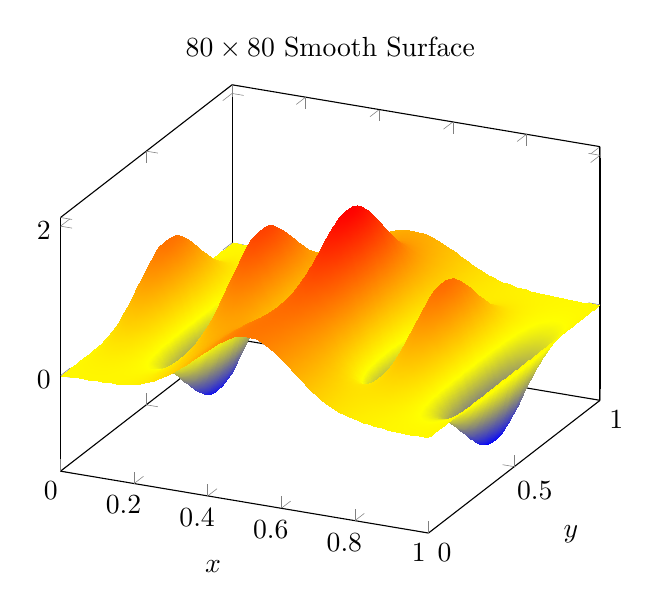
\begin{tikzpicture}
\begin{axis}[
	title=$80 \times 80$ Smooth Surface,
	xlabel=$x$,
	ylabel=$y$]
\addplot3[surf,samples=80,shader=interp,domain=0:1] 
	{sin(deg(8*pi*x))* exp(-20*(y-0.5)^2) 
	+ exp(-(x-0.5)^2*30 
		- (y-0.25)^2 - (x-0.5)*(y-0.25))};
\end{axis}
\end{tikzpicture}
\end{codeexample}

\PGFPlots\ relies completely on \TeX\ to do all typesetting. It uses the front-end-layer and basic layer of \PGF\ to perform all drawing operations. For complicated plots, this may take some time, and you may want to read Section~\ref{sec:pgfplots:importexport} for how to write single figures to external graphics files. Externalization is the best way to reduce typesetting time.

However, for large scale plots with a lot of points, limitations of \TeX's capacities are reached easily.

\subsection{Memory Limitations}
The default settings of most \TeX-distributions are quite restrictive, so it may be necessary to adjust them. 

Usually, the log--file or the final error message contains a summary about the used resources, giving a hint which parameter needs to be increased.

\subsubsection{LuaLa\TeX}
One solution which works quite well is to switch the La\TeX\ executable: if you have a decent \TeX\ distribution, you will have the |lualatex| executable as well. This, in turn, uses dynamic memory allocation such that it usually has enough memory for any \PGFPlots\ axis.

The LuaLa\TeX\ executable |lualatex| is supposed to be almost compatible with |pdflatex|. 

This approach works for any platform.

\subsubsection{Mik\TeX}
If you are running Mik\TeX\ and you do not want to (or cannot switch) to |lualatex|, you can proceed as follows.

For Mik\TeX, memory limits can be increased in two ways. The first is to use command line switches:
\begin{codeexample}[code only]
pdflatex 
	--stack-size=n --save-size=n 
	--main-memory=n --extra-mem-top=n --extra-mem-bot=n
	--pool-size=n --max-strings=n 
\end{codeexample}
\noindent Experiment with these settings if Mik\TeX\ runs out of memory. Usually, one doesn't invoke |pdflatex| manually: there is a development aid which does all the invocations, so this one needs to be adjusted. 

Sometimes it might be better to adjust the Mik\TeX\ configuration file permanently, for example to avoid reconfiguring the \TeX\ development program. This can be implemented using the command
\begin{codeexample}[code only]
initexmf --edit-config-file=pdflatex
\end{codeexample}
\noindent which can be typed either on a command prompt in Windows or using Start $\gg$ Execute. As a result, an editor will be opened with the correct config file. A sample config file could be
\begin{codeexample}[code only]
main_memory=90000000
save_size=80000
\end{codeexample}
or any of the config file entries which are listed below can be entered. 
Thanks to ``LeSpocky'' for his documentation in

\url{http://blog.antiblau.de/2009/04/21/speicherlimits-von-miktex-erhoehen}.

\subsubsection{\TeX Live or similar installations}
In addition to the option to switch to |lualatex|, you can proceed as follows to keep existing |dvips| or |pdflatex| workflows.

For Unix installations, one needs to adjust config files. This can be done as follows:
\begin{enumerate}
	\item Locate |texmf.cnf| on your system. On my Ubuntu installation, it is in 
	
	|/usr/share/texmf/web2c/texmf.cnf|.
	\item Either change |texmf.cnf| directly, or copy it to some convenient place. If you copy it, here is how to proceed:
		\begin{itemize}
			\item keep only the changed entries in your local copy to reduce conflicts. \TeX\ will always read \emph{all} config files found in its search path.
			\item Adjust the search path to find your local copy. This can be done using the environment variable |TEXMFCNF|. Assuming your local copy is in |~/texmf/mytexcnf/texmf.cnf|, you can write
\begin{codeexample}[code only]
export TEXMFCNF=~/texmf/mytexcnf:
\end{codeexample}
			to search first in your directory, then in all other system directories.
		\end{itemize}
	\item You should change the entries
\begin{codeexample}[code only]
main_memory = n
extra_mem_top = n
extra_mem_bot = n
max_strings = n
param_size = n
save_size = n
stack_size = n
\end{codeexample}
		The log--file usually contains information about the parameter which needs to be enlarged.
\end{enumerate}
An example of this config file thing is shown below. It changes memory limits.
\begin{enumerate}
	\item Create the file |~/texmf/mytexcnf/texmf.cnf| (and possibly the paths as well).
\begin{codeexample}[code only]
% newly created file ~/texmf/mytexcnf/texmf.cnf:
% If you want to change some of these sizes only for a certain TeX
% variant, the usual dot notation works, e.g.,
% main_memory.hugetex = 20000000
main_memory = 230000000 % words of inimemory available; also applies to inimf&mp
extra_mem_top = 10000000     % extra high memory for chars, tokens, etc.
extra_mem_bot = 10000000     % extra low memory for boxes, glue, breakpoints, etc.
save_size = 150000	% for saving values outside current group
stack_size = 150000	% simultaneous input sources

% Max number of characters in all strings, including all error messages,
% help texts, font names, control sequences.  These values apply to TeX and MP.
%pool_size = 1250000
% Minimum pool space after TeX/MP's own strings; must be at least
% 25000 less than pool_size, but doesn't need to be nearly that large.
%string_vacancies = 90000
% Maximum number of strings.
%max_strings = 100000
% min pool space left after loading .fmt
%pool_free = 47500
\end{codeexample}
	\item Run |texhash| such that \TeX\ updates its |~/texmf/ls-R| database.
	\item Create the environment variable |TEXMFCNF| and assign the value `|~/texmf/mytexcnf:|' (including the trailing `|:|'!). For my linux system, this can be done using by adding
\begin{codeexample}[code only]
export TEXMFCNF=~/texmf/mytexcnf:
\end{codeexample}
	to |~/.bashrc|.
\end{enumerate}

Unfortunately, \TeX\ does not allow arbitrary memory limits, there is an upper bound hard coded in the executables.

\subsection{Reducing Typesetting Time}
\PGFPlots\ does a lot of computations ranging from abstract coordinate computations to low level |.pdf| drawing commands (implemented by \PGF). For complex plots, this may take a considerable time -- especially for 3D plots.

One possibility to reduce typesetting time is to tell \PGF\ to generate single, temporary |.pdf| (or |.eps|) documents for a subset (or all) graphics in one run and re-use these temporary images in successive runs. For \PGFPlots, this is the most effective way to reduce typesetting time. It can be accomplished using the |external| library described in Section~\ref{sec:pgfplots:export}.
}
